\documentclass[a4paper,10 pt]{article}
\usepackage{geometry}
\geometry{letterpaper, margin=0.8in}
\usepackage[english]{babel}
\usepackage[utf8]{inputenc}
\usepackage{amsmath}
\usepackage{graphicx}
\usepackage[colorinlistoftodos]{todonotes}
\usepackage{float}
\usepackage[numbered]{mcode}
\renewcommand{\baselinestretch}{1.1}

\title{Instruments of Time-Frequency Analysis: The G\'abor Transform, Applied to Music}

\author{Dana Korssjoen} 

\date{12 February 2020}

\begin{document}
\maketitle
\begin{abstract}
    This report applies the G\'abor transform and various periodic window functions to analyze several audio signals across multiple features. The ultimate goal of this time-frequency analysis is to describe a sample from Handel's \emph{Messiah} in a quantitative way, discuss the differences in timbre of two different instruments (piano and recorder), and reproduce a music score from a simple audio sample of the song Mary Had a Little Lamb.
\end{abstract}
\section{Introduction and Overview}

This report applies time-frequency analysis tools to identify key aspects of audio recordings. In particular, it uses the G\'abor transform and other window functions as primary analytical tools. The two main tasks carried out in this report are: Task I, which is concerned with applying these tools to explore key features of a recording of Handel's Messiah; and Task II, which applies time-frequency analysis to compare the timbre of two different instruments and ascertain which notes they are playing in a simple audio recording.

\section{Theoretical Background}
The techniques used in this report heavily rely on the use of the Fast Fourier transform to convert signals from the time domain to the frequency domain. However, because the theoretical background for the FFT was covered extensively in the last report, I will assume that the reader is familiar with it.

Instead, I will describe the theoretical background of the G\'abor transform, which is a discrete, windowed modification of the Fourier transform kernel. Under this modification, the G\'abor transform is defined as 
\begin{equation}
    \mathcal{G}[f](t,\omega)=\int_{-\infty}^\infty f(\tau)g(\tau-t)e^{-i\omega\tau}d\tau
\end{equation}
where $g(\tau-t)$ is a window function that localizes the Fourier integral around $t=\tau$. When I speak of the G\'abor transform in general in this report, I mean it in the context of the Gaussian window function, which is
\begin{equation}
    g(\tau-t)=e^{-(t-\tau)^2}
\end{equation}
There are lots of other functions that can be used, however, as I will demonstrate in this report. Two such functions are the Mexican Hat filter, so called because it resembles a sombrero. Its equation is
\begin{equation}
    \phi(t-\tau)=(1-(t-\tau)^2)e^{-(t-\tau)^2/2}
\end{equation}
There is also the Shannon filter, which is a simple step function defined as
\begin{equation}
    \phi(t-\tau)=\begin{cases}1 & t-\tau \leq 1/2 \\ 0 & t-\tau > 1/2\end{cases}
\end{equation}
The advantage of G\'abor analysis is to achieve better resolution in time versus a Fourier analysis, while also achieving better resolution in frequency than times series analysis. The specifics of this tradeoff can be manipulated by shrinking the width of the filter window, which yields better time resolution but poorer frequency resolution. In particular, smaller windows may not be able to capture low-frequency information.

In this report, I apply both under-sampling and over-sampling to demonstrate the impact of the choice in sampling method. Over-sampling refers the practice of making small translation steps in time so that the filter windows are overlapping. This produces some redundancy of information, but captures more details. Under-sampling occurs in the opposite circumstance - when the translation step is large enough that windows do not overlap.

The final piece of theoretical background that is needed in this report is a rudimentary understanding of music and instrumentation. The key thing to understand, is that musical notes are defined by their frequencies. Table 1 shows the frequency in Hertz of a selected group of musical notes\cite{MTU}. The other key thing to understand here is \emph{timbre}. Timbre refers to the characteristic set of overtones that give a musical instrument its unique sound. In other words, timbre is what causes a piano and a recorder to sound distinct when making the same note. A key component of timbre, harmonic overtones refer to notes that are a integer multiple of the fundamental frequency being produced\cite{MVCC}. The structure of overtones can also vary across instruments, meaning that even if the same overtones sound, they may not necessarily have the same relative volumes.
\begin{table}[]
\begin{tabular}{llllllllllll}
Note      & B_3   & C_4   & C\#_4 & D_4   & D\#_4 & E_4   & F_4   & F\#_4 & G_4   & G\#_4 & A_4 \\
Freq (Hz) & 246.94 & 261.63 & 277.18 & 293.66 & 311.13 & 329.63 & 349.23 & 369.99 & 392.00 & 415.30 & 440.00
\end{tabular}
\caption{Hz Frequency of Selected Music Notes}
\end{table}
With that background established, it's time to move into discussion of the algorithm used in this report.
\section{Algorithm Implementation and Development}
\subsection{Task I: Analysis of Handel's Messiah}
The first task is loading the data and creating the appropriate variables for time-frequency analysis. This is completed in lines 1-20 in Section 7.1 of this report. As always, it's important to scale frequencies by $2*\pi/L$ because Fourier transform uses pi-periodicity. It's also important to apply fftshift to the frequency vector to match the output of the Fourier transform.

Lines 22-41 are used to generate and plot the G\'abor transform with window width coefficients of 100, 10, 1 and 0.1, in order. To do this, we take multiply our signal by the Gaussian filter with the appropriate window width and center in time, then find its Fourier transform. We do this in steps of .1 to generate a spectrogram with high resolution in both time and frequency. This is over-sampling. The results are seen in Figure 1.

Lines 43-96 are used to generate and plot the signal with different window functions applied: G\'abor, Mexican, and Shannon, respectively. Each has window width coefficient of $30$ and a translation step of $.1$, so we are still significantly over-sampling. As above, we simply construct the filter, center it at the appropriate point in time, multiply our signal by it, and take the Fourier transform. The results are shown in Figure 2.
\subsection{Task II: Instrument Comparison}
As before, we begin in lines 1-14 by initializing the values, remember to scale and shift our frequencies to be compatible with the Fourier transform. Lines 16-28 generate the vectors needed to plot the spectrogram, using the same process as outlined in Task I. A window width coefficient of 100 and translation step of .1 was chosen through experimentation. The vector needed for the pseudo-score is also generated in this section - it will be discussed in a later paragraph.

Lines 30-57 complete the same tasks, except for the recording made by the recorder.

Lines 59-74 generate the spectrogram, again as outlined in Task I. The results are shown in Figure 3.

Lines 76-109 plot the pseudo-score for this piece of music. It was generated on lines 25-26 and 54-55 according to the following algorithm: at each point in time, find the maximum in the Fourier transformed data. The index at which this occurs corresponds to the frequency at which the signal is most intense at this point in time - the center frequency. Save this center frequency at every point measured to recover the score. Figure 4 shows these frequencies plotted in time, with lines overlaying the characteristic frequencies of each musical note.
\section{Computational Results}
\subsection{Task I: Analysis of Handel's Messiah}
The spectrograms generated by different window widths on the Gaussian filter are shown in Figure 1. As anticipated, higher values of $a$ create narrower windows, which increases time resolution. The narrowest window, $a=100$, in Figure 1 displays very time-localized data, whereas $a=0.1$ generated almost continuous lines across the entire time window, nearly resembling a Fourier transform.

In Figure 2, we see the results of different types of filters. It appears that the Gaussian filter and Mexican Hat filter perform similar at these parameters ($a=100, t\_step=.1$), with the Gaussian filter perhaps slightly outperforming in terms of frequency resolution, while the Shannon filter has much poorer time resolution. This makes sense when you think about the shape of the filters - as a step function, the Shannon filter is a much blunter instrument of analysis than the Gaussian or Mexican Hat filters, which are better at amplifying a center frequency. In fact, these two filters are very precise with a narrow window width like this, so it makes sense that we see such high resolution.

In all three spectrograms, we can see the presence of ample overlapping frequencies and overtones. The Shannon filter in particular gives us a good sense of how rich this audio signal is with different frequencies. Now, to discuss overtones in more depth, we move to Task II.
\begin{figure}[H]
  \centering
    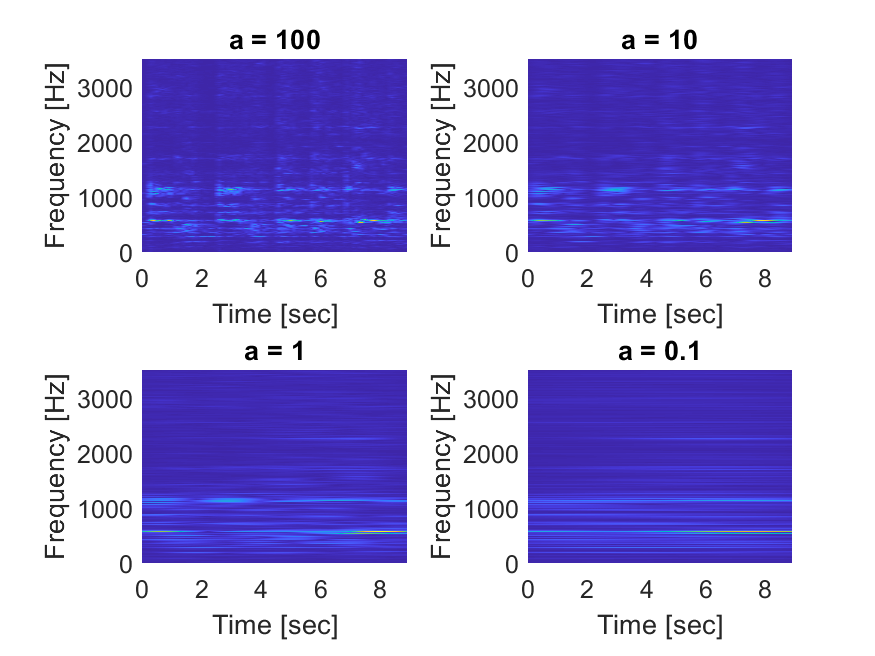
\includegraphics[width = .9\textwidth]{hw2/images/p1-windows.png}
    \label{fig:windows1}
    \caption{The G\'abor transform with specified window parameters}
\end{figure}

\begin{figure}[H]
  \centering
    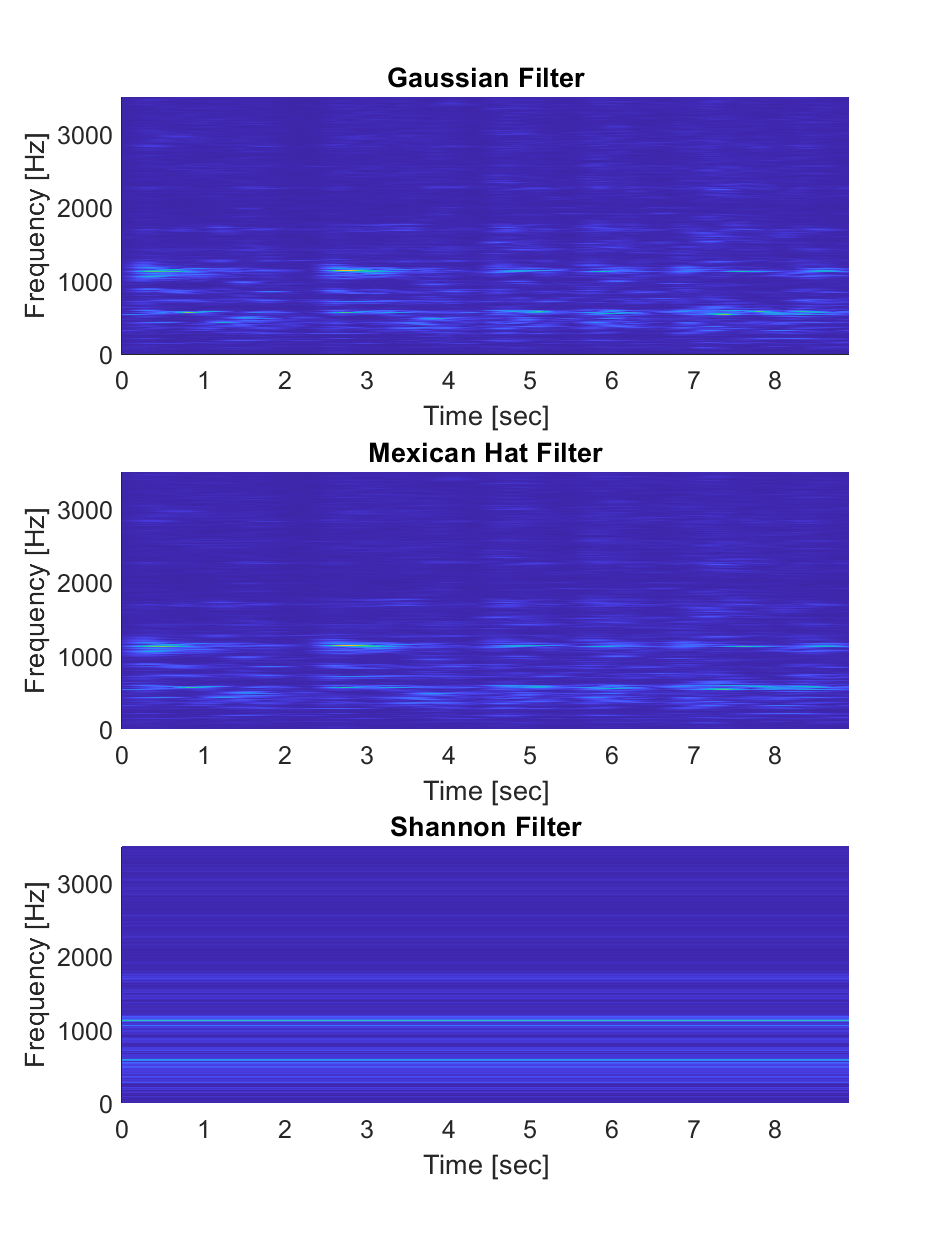
\includegraphics[width = .75\textwidth]{hw2/images/p1-functions.png}
    \label{fig:functions1}
    \caption{Use of different window functions}
\end{figure}
\subsection{Task II: Instrument Comparison}
This task focuses on identifying the notes played, and difference in timbre, between two instruments: the piano and the recorder. In Figure 3, we see the spectrograms for these two instruments. In general, we see that they are playing similar lines with similar rhythms, though the actual notes are shifted upwards in the case of the recorder. Looking closely, we can see differences in the timbre of the two instruments. The piano has more residual frequencies clustered just above and below its fundamental frequencies, suggesting an audibly richer sound, as well as a greater volume of mid-range overtones, and fainter high-range overtones than the recorder. In contrast, the recorder has a relatively precise timbre, with few tones clustered around its fundamental frequencies, but more intense high-range overtones. It is likely the presence of these higher-frequency overtones that gives the recorder its signature tinny, almost whiny sound.

In Figure 4, we can view the reproduced pseudo-scores for each of these instruments. As in the spectrograms, it is clear that the piano and recorder are playing the same melodic line, but the recorder is playing at a higher pitch. In particular, the piano uses the notes E4, D4, and C4, while the recorder uses B4, A4, and G4.

\begin{figure}[H]
  \centering
    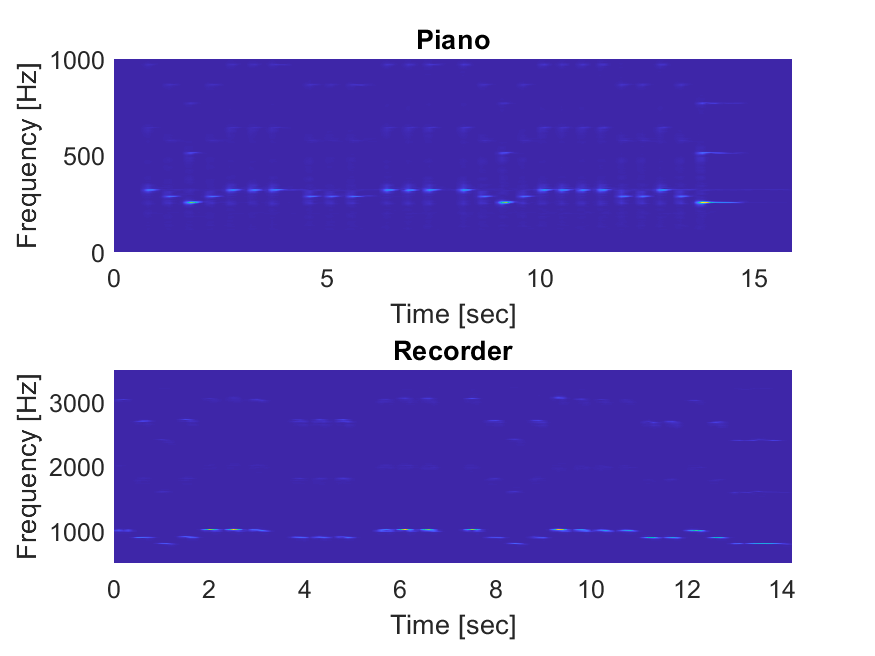
\includegraphics[width = .75\textwidth]{hw2/images/p2-spectrograms.png}
    \label{fig:spec2}
    \caption{Spectrograms for the two instruments}
\end{figure}

\begin{figure}[H]
  \centering
    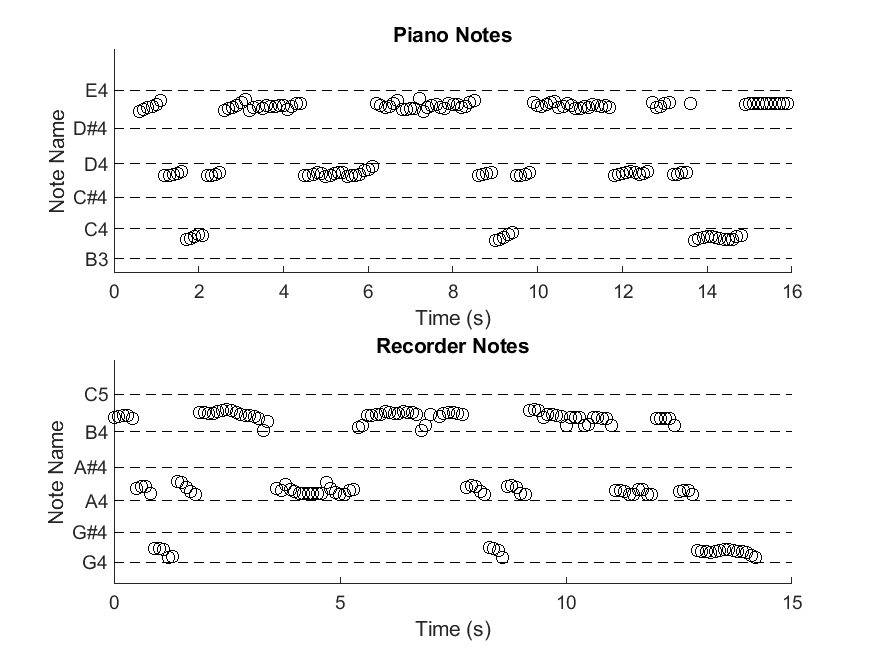
\includegraphics[width = .7\textwidth]{hw2/images/p2-notes.png}
    \label{fig:notes}
    \caption{Musical notes in time for each instrument}
\end{figure}
\section{Summary and Conclusions}
In this report, we used the G\'abor transform with a variety of window sizes and window functions to examine audio recordings. Using these techniques, we were able to analyze the musical effect of the snippet of Handel's Messiah, discuss the timbre of the two instruments examined, and recover a pseudo-score of the music played, which was "Mary Had a Little Lamb." This report is an example of the broad variety of applications of time-frequency analysis tools, and serves as an example of the importance of experimenting with different parameters and filters to find which suits your data best. Used carefully, these tools work in perfect harmony with the signal data they are applied to.
\section{Appendix A: MATLAB Functions and Implementation}
\begin{table}[H]
\begin{tabular}{ll}
plot(x,y) & generates a 2-dimensional line plot \\
xlabel/ylabel() & used to edit x/y labels on the current plot (resp.) \\
title() & used to edit title of the current plot \\
saveas() & saves the specified figure to a file \\
length() & returns the integer length of the specified vector \\
linspace(start,end,n) & returns a vector of n linearly spaced points from start to end \\
fftshift(A) & shifts the zero-frequency component of $A$ to the center of $A$ \\
zeros() & returns a vector of all zeros of the specified dimensions \\
exp(x) & the Matlab expression for the function e^x \\
fft() & performs the Fast Fourier Transform \\
abs() & returns the absolute value of the input \\
subplot() & generates a matrix of figures of the specified size \\
pcolor() & used for generating spectrograms - uses the matrix data to produce an array of colored cells \\
audioread() & returns the sampled data and sample rate from the specified file \\
{[}M,I{]} = max() & returns the maximum value (M) and the index at which it occurs (I) in the input \\
scatter() & produces a scatter plot of the inputted data \\
yticks() & used to add ticks at the specified points on the y axis \\
yticklabels() & used to add labels to yticks, created with above function \\
 &  \\
 & 
\end{tabular}
\end{table}
\newpage
\section{Appendix B: MATLAB Code}
\subsection{Part I: Analysis of Handel's Messiah}
\begin{lstlisting}
%% prepare variables
clear; close all;
load handel
v = y';
plot((1:length(v))/Fs,v);
xlabel('Time [sec]');
ylabel('Amplitude');
title('Signal of Interest, v(n)');
%p8 = audioplayer(y,Fs);
%playblocking(p8);
saveas(gcf,'p1-rawdata.png')

% initialize
S = v;
n = length(v);
L = n/Fs; % time in seconds
t = linspace(0,L,n+1);
t = t(1:n);
k = (2*pi/L)*[0:(n-1)/2 -(n-1)/2:-1];
ks = fftshift(k);

%% vary window width
a_vec = [100 10 1 0.1];
for jj = 1:length(a_vec)
    a = a_vec(jj);
    tslide=0:0.1:L;
    Sgt_spec = zeros(length(tslide),n);
    for j=1:length(tslide)
        g=exp(-a*(t-tslide(j)).^2);
        Sg=g.*S;
        Sgt=(fft(Sg));
        Sgt_spec(j,:) = fftshift(abs(Sgt));
    end
    subplot(2,2,jj);
    pcolor(tslide,ks/(2*pi),Sgt_spec.'), shading interp
    title(['a = ',num2str(a)],'Fontsize',12)
    xlabel('Time [sec]')
    ylabel('Frequency [Hz]')
    set(gca,'Ylim',[0 3500],'Fontsize',12)
end
saveas(gcf,'p1-windows.png')

%% change window function
% init fixed values
tslide = 0:.1:L;
a = 30;

% gabor
Sgabor_spec = zeros(length(tslide),n);
for j=1:length(tslide)
    gabor = exp(-a*(t-tslide(j)).^2);
    Sgabor = fft(S.*gabor);
    Sgabor_spec(j,:) = fftshift(abs(Sgabor));
end

% mexican hat
S_mex_spec = zeros(length(tslide),n);
for j=1:length(tslide)
    mex_hat = (1 - (t-tslide(j)).^2).*(exp(-a*(t-tslide(j)).^2/2));
    S_mex = fft(S.*mex_hat);
    S_mex_spec(j,:) = fftshift(abs(S_mex));
end

% shannon
S_shan_spec = zeros(length(tslide),n);
for j=1:length(tslide)
    shannon = (abs(t-tslide(j)) <= a/2);
    S_shan = fft(S.*shannon);
    S_shan_spec(j,:) = fftshift(abs(S_shan));
end

% plot
figure('Position',[500, 0, 600, 800])

subplot(3,1,1)
pcolor(tslide,ks/(2*pi),Sgabor_spec.'), shading interp
title(['Gaussian Filter'],'Fontsize',12)
xlabel('Time [sec]');
ylabel('Frequency [Hz]');
set(gca,'Ylim',[0 3500],'Fontsize',12)

subplot(3,1,2)
pcolor(tslide,ks/(2*pi),S_mex_spec.'), shading interp
title(['Mexican Hat Filter'],'Fontsize',12)
xlabel('Time [sec]');
ylabel('Frequency [Hz]');
set(gca,'Ylim',[0 3500],'Fontsize',12)

subplot(3,1,3)
pcolor(tslide,ks/(2*pi),S_shan_spec.'), shading interp
title(['Shannon Filter'],'Fontsize',12)
xlabel('Time [sec]');
ylabel('Frequency [Hz]');
set(gca,'Ylim',[0 3500],'Fontsize',12)

saveas(gcf,'p1-functions.png')
\end{lstlisting}
\subsection{Part II: Instrument Comparison}
\begin{lstlisting}
%% piano
[y,Fs] = audioread('music1.wav');
tr_piano=length(y)/Fs; % record time in seconds
%p8 = audioplayer(y,Fs);
%playblocking(p8);

% init
S = y';
n = length(y);
L = tr_piano;
t = linspace(0,L,n+1);
t = t(1:n);
k = (2*pi/L)*[0:(n/2-1) -n/2:-1];
ks_p = fftshift(k);

% prep spectrogram
a = 100;
tslide_p=0:.1:L;
p_notes = zeros(1,length(tslide_p));
Sgt_spec_p = zeros(length(tslide_p),n);
for j=1:length(tslide_p)
    g=exp(-a*(t-tslide_p(j)).^2);
    Sg=g.*S;
    Sgt=(fft(Sg));
    [M,I] = max(fftshift(abs(Sgt)));
    p_notes(j) = abs(ks_p(I))/(2*pi);
    Sgt_spec_p(j,:) = fftshift(abs(Sgt));
end

%% recorder
[y,Fs] = audioread('music2.wav');
tr_rec=length(y)/Fs; % record time in seconds
%p8 = audioplayer(y,Fs);
%playblocking(p8);

% init
S = y';
n = length(y);
L = tr_rec; % time in seconds
t = linspace(0,L,n+1);
t = t(1:n);
k = (2*pi/L)*[0:(n/2-1) -n/2:-1];
ks_r = fftshift(k);

% prep spectrogram
a = 100;
tslide_r=0:.1:L;
r_notes = zeros(1,length(tslide_r));
Sgt_spec_r = zeros(length(tslide_r),n);
for j=1:length(tslide_r)
    g=exp(-a*(t-tslide_r(j)).^2);
    Sg=g.*S;
    Sgt=(fft(Sg));
    [M,I] = max(fftshift(abs(Sgt)));
    r_notes(j) = abs(ks_r(I))/(2*pi);
    Sgt_spec_r(j,:) = fftshift(abs(Sgt));
end

%% generate spectrograms
subplot(2,1,1)
pcolor(tslide_p,ks_p/(2*pi),Sgt_spec_p.'), shading interp
title('Piano')
xlabel('Time [sec]')
ylabel('Frequency [Hz]')
set(gca,'Ylim',[0 1000],'Fontsize',12)

subplot(2,1,2)
pcolor(tslide_r,ks_r/(2*pi),Sgt_spec_r.'), shading interp
title('Recorder')
xlabel('Time [sec]')
ylabel('Frequency [Hz]')
set(gca,'Ylim',[500 3500],'Fontsize',12)

saveas(gcf,'p2-spectrograms.png')

%% generate score
subplot(2,1,1)
for j=1:length(p_notes)
    scatter(tslide_p(j), p_notes(j),'k')
    hold on
end
p_note_names = [246.94, 261.63, 277.18, 293.66, 311.13, 329.63];
for j=1:length(p_note_names)
    plot([0 16],[p_note_names(j) p_note_names(j)],'k--')
end
yticks(p_note_names)
yticklabels({'B3','C4','C#4','D4','D#4','E4'})
title('Piano Notes')
ylabel('Note Name')
xlabel('Time (s)')
set(gca,'Ylim',[240 350])

subplot(2,1,2)
for j=1:length(r_notes)
    scatter(tslide_r(j), r_notes(j),'k')
    hold on
end
r_note_names = [783.99, 830.61, 880, 932.33, 987.77, 1046.5];
for j=1:length(r_note_names)
    plot([0 15],[r_note_names(j) r_note_names(j)],'k--')
end
yticks(r_note_names);
yticklabels({'G4','G#4','A4','A#4','B4','C5'});
title('Recorder Notes')
ylabel('Note Name')
xlabel('Time (s)')
set(gca,'Ylim',[750 1100])

saveas(gcf,'p2-notes.png')
\end{lstlisting}
\begin{thebibliography}{9}
\bibitem{MTU} "Physics of Music - Notes." Michigan Tech University. https://pages.mtu.edu/~suits/notefreqs.html

\bibitem{MVCC} Prof. Fiore. "Pitch, Frequency, Overtones, Timbre and All That Stuff." Mohawk Valley Community College. https://www2.mvcc.edu/users/faculty/jfiore/SoS/work/Overtones.pdf

\end{thebibliography}
\end{document}